\section{Versuchsauswertung}

\subsection{Versuch 1}
Im ersten Versuchsteil wurden sechs verschiedene Durchflüsse von \SI{60}{\liter\per\hour} bis \SI{660}{\liter\per\hour} mit Hilfe eines Taco-Setters eingestellt und die Messdaten der verbauten Sensoren verglichen. Als Referenz wurde das durchströmende Wasser am Auslass der Messstrecke in einem Eimer gesammelt, gewogen und die Messdauer notiert. Dieser Wert wird als wahrer Durchfluss angenommen. Abbildung \ref{fig:devPc} zeigt die Abweichung der unterschiedlichen Sensoren vom Wahren Durchfluss. 
\begin{figure}[H]
	\centering
	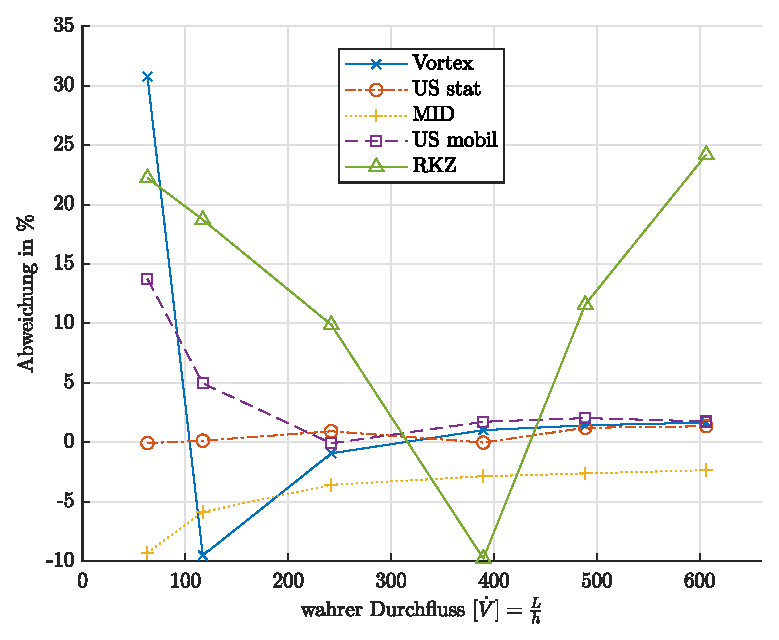
\includegraphics[width=0.8\textwidth]{../DATA/devPcPlot.eps}
	\caption[bla]{bla}
	\label{fig:devPc}
\end{figure}

\begin{table}[H]
	\centering
	\caption{Arithmetische Mittelwerte und Standardabweichung der Durchflussensoren.}
	\label{tab:meanSigData}
	\begin{tabular}{S[separate-uncertainty,table-parse-only,table-figures-uncertainty = 1]S[separate-uncertainty,table-parse-only,table-figures-uncertainty = 1]S[separate-uncertainty,table-parse-only,table-figures-uncertainty = 1]S[separate-uncertainty,table-parse-only,table-figures-uncertainty = 1]}
		
		
		
		{wahrer Durchfluss}        &  {Vortex}            &{US stat}            &{MID}            \\  
		63.14220               &  43.7156  (243188  ) & 63.1847  (  10577) &  69.0083  ( 06710 )  \\
		116.9762               &  128.1026 ( 09770  ) & 116.8114 (  10102) &  123.8232 ( 08339 )  \\
		241.8581               &  244.0911 ( 11393  ) & 239.6007 (  10094) &  250.4983 ( 09285 )  \\
		389.7605               &  385.7592 ( 25079  ) & 389.8219 (195831)  & 400.8603 ( 22251 )   \\
		488.8910               &  481.8952 ( 18571  ) & 482.9031 (  15359) &  501.6424 ( 13441 )  \\
		606.4940               &  596.3836 ( 28746  ) & 598.2423 (  27780) &  620.5848 ( 33006 )  \\
		\hline
		{wahrer Durchfluss}&		{US mobil}       &    {RKZ}           				 & \\
		63.14220						&		54.4603   ( 14218 ) &  49.1009  ( 181448) 		 & \\
		116.9762						&		111.1667  ( 12612 ) &   95.0675  ( 350284) & \\
		241.8581						&		242.0576  ( 08049 ) &  217.9288  ( 677619) & \\
		389.7605						&		383.0093  ( 30340 )  & 427.8585  (1323540) & \\
		488.8910						&		478.9012  ( 19726 ) &  432.1874  (1361169) & \\
		606.4940						&		595.8492  ( 31063 ) &  459.7167  (1865268) & \\
		
	\end{tabular}
\end{table}


Die geringste Abweichung bietet das Stationäre Ultraschallgerät mit unter 2\% Abweichung über den gesamten Messbereich hinweg. Auch das mobile Ultraschallgerät bietet ab \SI{240}{\liter\per\hour} eine ähnliche Genauigkeit. Das MID bietet erst ab einem Durchfluss von \SI{300}{\liter\per\hour} eine konstante Genauigkeit bei einer Abweichung von -3\%. Der Vortexmesser ist mit einem minimalen Arbeitsbereich von \SI{50}{\liter\per\hour} angegeben, praktisch liefert er bei \SI{60}{\liter\per\hour} keinen brauchbaren Wert. Ab \SI{240}{\liter\per\hour} liefert er plausible Werte. Am schlechtesten schneidet der Ringkolbenzähler ab, welcher mit hohen Abweichungen im zweistelligen Bereich (je nach Durchflussrate in beide Richtungen) lediglich für qualitative Messungen geeignet ist.

\subsection{Versuch 2}

%Tabelle mit den Messwerten anlegen

Abbildung \ref{fig:temp} zeigt den gemessenen Temperaturverlauf der beiden Sensoren.
\begin{figure}[H]
	\centering
	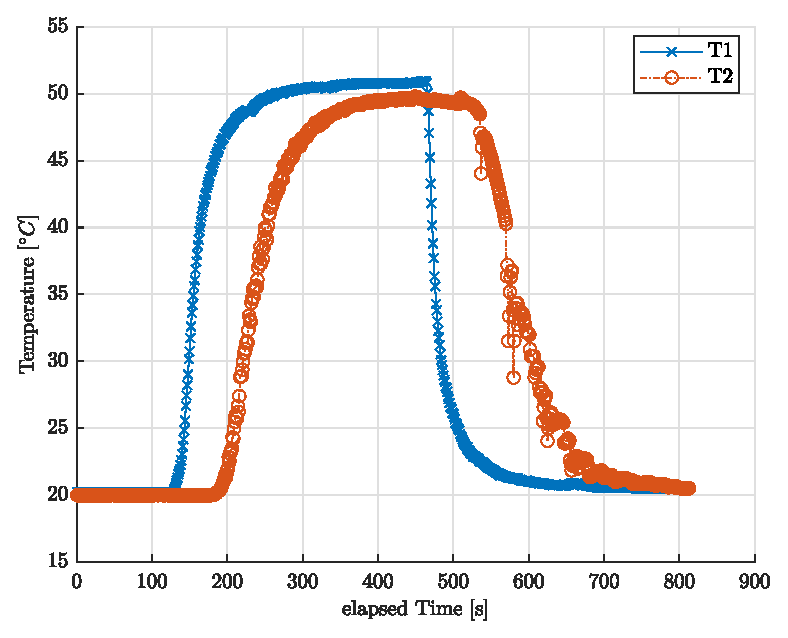
\includegraphics[width=0.8\textwidth]{../DATA/tempPlot.eps}
	\caption[bla]{bla}
	\label{fig:temp}
\end{figure}

Zur Bestimmung des Durchflusses wird  die Laufzeit (Zeitlicher Abstand der Flanken beider Verläufe) bestimmt. Dieser ist ABbildung \ref{fig:temp} zu entnehmen.

\begin{center}
	\begin{tabular}{l|c}
		\label{tab:}
		
		\textbf{Flanke} & \textbf{Laufzeit} [s]\\
		\hline
		steigend & x \\
		fallend & y \\
	\end{tabular}
\end{center}
%%%%%% exakte Flankenabstände einsetzen
Für die Auswertung wird die steigende Flanke genutzt, da diese schärfer aufgelöst ist.

Die gemessene Strecke zwischen den beiden Sensoren beträgt \SI{9,48}{\meter}, der Querschnitt der Leitung ist mit \SI{0,02}{\meter} angegeben. Das Volumen der Messstrecke berechnet sich nach Gleichung \ref{eq:vol} zu:

\begin{equation}
	\label{eq:vol}
	V_{Rohr} = \pi * r^2 * l = \pi * (\SI{0,01}{\meter})^2 * \SI{9,48}{\meter} = \SI{2,978}{\liter}
\end{equation}

Der Durchfluss entspricht dem Quotienten aus Rohrvolumen und Laufzeit und ist in Gleichung \ref{eq:flow} berechnet.

\begin{equation}
	\label{eq:flow}
	\dot V = \frac{V_{Rohr}}{t_{LZ}}*\SI{3600}{\second\per\hour} = \frac{\SI{2,978}{\liter}}{\SI{75}{\second}}*\SI{3600}{\second\per\hour} = \SI{142,9}{\liter\per\hour}
\end{equation}

%%%%%%in Gleichung 2 exakten Abstand FLanke einsetzen und Berechnen
%%%%%%%Messwert MID vergleichen.

